% LTeX: language=en-GB
%Author(s), Course variables
\newcommand{\titl}{02132 Assignment 3 report}
\newcommand{\subtitl}{Implementation of an FSMD-based hardware\\accelerator for the image erosion in Chisel}
\newcommand{\authone}{Niclas Juul Schæffer}
\newcommand{\SIDone}{s224744}
\newcommand{\authtwo}{Rasmus Kronborg Finnemann Wiuff}
\newcommand{\SIDtwo}{s163977}
\newcommand{\lb}{\\}
%Basics
\documentclass[a4paper, english]{article}
\usepackage[utf8]{inputenc}
\usepackage[T1]{fontenc}
\usepackage[bitstream-charter]{mathdesign}
\usepackage{babel}
\usepackage[moderate, mathspacing=normal]{savetrees}
%Symbols and scientifics
\usepackage{bm}
\usepackage{physics}
\usepackage{mathtools}
\numberwithin{equation}{section}
% \usepackage{siunitx}
% \sisetup{
% per-mode = power ,
% round-mode = figures ,
% round-precision = 3 ,
% exponent-mode = input ,
% output-decimal-marker = {.} ,
% exponent-product = 	imes ,
% uncertainty-mode = separate ,
% range-phrase = - ,
% range-units =  single ,
% inter-unit-product = \ensuremath{{\cdot{}}} ,
% quantity-product = \ ,
% separate-uncertainty-units = single ,
% }

%Appendix, TOC and Bibliography
\usepackage{appendix}
\renewcommand\appendixtocname{Appendix}
\usepackage[nottoc]{tocbibind}
\setcounter{tocdepth}{2}
\usepackage{lastpage}

%Figures
\usepackage[svgnames]{xcolor} % Required to specify font color
\usepackage{float}
\usepackage{graphicx}
\usepackage{subcaption}
\usepackage[format=plain,
    labelfont={bf,it,footnotesize},
    textfont={it,footnotesize}]{caption}
% \captionsetup[table]{name=Huskeord}
\captionsetup{font={stretch=0.9}}
\usepackage{wrapfig}
\usepackage[a4paper, centering, rmargin=2.5cm, tmargin=2.5cm, lmargin=2.5cm, bmargin=3.5cm]{geometry}
\usepackage{verbatim}
\usepackage[space]{grffile}
\usepackage[final]{pdfpages}
\usepackage{pdflscape}
\usepackage{multirow}
\usepackage{fontawesome}
\usepackage{tikz}
\usepackage{pgfgantt}
% \usetikzlibrary{external}
% \tikzexternalize[prefix=tikz/]
% \usepackage{circuitikz}
% \ctikzset{logic ports = ieee}
\usetikzlibrary{positioning,arrows,automata}
% \newcommand{\pin}[3]{\node[blue, font = \small, #2] at (#1) {#3};
                    %  \coordinate (#3) at (#1);}
% \newcommand{\port}[4]{\node[circ, #2] (#1) {};
                    %  \node[#3] at (#1) {#4};}
%Header footer
\usepackage{fancyhdr}
\pagestyle{fancy}
\lhead{02132 Computer Systems \lb Assignment 3 \lb December \nth{1}}
\chead{
\includegraphics[width=.05\textwidth]{DTU}}
\rhead{Group 22 \lb \authone \ \textbf{\SIDone} \lb \authtwo \ \textbf{\SIDtwo}}
\cfoot{Page \thepage\, of\, \pageref*{LastPage}}
\renewcommand{\headrulewidth}{0.4pt}
\renewcommand{\footrulewidth}{0.4pt}
\setlength{\headheight}{36.75034pt}

%Text tools
\usepackage{listings}
\usepackage{parcolumns}
\usepackage[super]{nth}
\usepackage[normalem]{ulem}
\usepackage{import}
\usepackage{url}
\usepackage{lipsum}
\usepackage{microtype}
\usepackage[pdfencoding=auto, psdextra]{hyperref}
\hypersetup{
    colorlinks   = true, %Colours links instead of ugly boxes
    urlcolor     = blue, %Colour for external hyperlinks
    linkcolor    = blue, %Colour of internal links
    citecolor   = red %Colour of citations
}
\usepackage[capitalise]{cleveref}
% \crefname{table}{Huskeord}{Huskeord}
\usepackage{enumitem}
\newlist{arrowlist}{itemize}{1}
\setlist[arrowlist]{label={\(\rightarrow\)}}
\usepackage{tabularray}
\UseTblrLibrary{booktabs}
\usepackage{todonotes}
\usepackage[square, longnamesfirst, numbers]{natbib}
\usepackage{empheq}
% \usepackage[newfloat, outputdir=/]{minted} % Overleaf minted buildpath fix
\usepackage[newfloat]{minted}
\setminted{fontsize=\small,
           linenos=true}
\usemintedstyle{tango}
\SetupFloatingEnvironment{listing}{listname=Listings}
\captionsetup[listing]{position=top, skip=-1pt}
% \newcommand{\im}[3]{\inputminted[linenos=true, python3=true, firstline=#2, lastline=#3]{python}{#1}}
% \newcommand{\java}[3]{\inputminted[linenos=true, firstline=#2, lastline=#3]{java}{#1}}
% \usepackage{dirtree}

%Definitions and new commands
\newcommand{\degr}{^{\circ}}
\newcommand{\me}{\mathrm{e}}

%Title and sectioning
\def\Vhrulefill{\leavevmode\leaders\hrule height 0.7ex depth \dimexpr0.4pt-0.7ex\hfill\kern0pt}
\usepackage{titlesec}
\usepackage{titling}
\definecolor{DTUred}{cmyk}{0, .91, .72, .23}
\definecolor{FMNgrey}{cmyk}{.73,.43,.53,.38}
%Use letters insted of numbers in section numbering
% \renewcommand{\thesection}{\Alph{section}}
% \renewcommand{\thesubsection}{\Alph{subsection}}

\makeatletter
\newcommand{\github}[1]{%
   \href{#1}{\color{DTUred}\faGithub}%
}
\makeatother

\begin{document}

\titleformat{\section}[block]
{\normalfont\Large\scshape\filright\color{DTUred}}{\fbox{\thesection}}{1em}{}

\titleformat{\subsection}
{\titlerule
    \vspace{.8ex}%
    \normalfont\scshape\color{FMNgrey}}
{\thesubsection.}{.5em}{}

\titleformat{\subsubsection}[wrap]
{\normalfont\fontseries{b}\selectfont\filright}
{\thesubsubsection.}{.5em}{}
\titlespacing{\subsubsection}
{12pc}{1.5ex plus .1ex minus .2ex}{1pc}

\title{\vspace{-40mm}\Huge\scshape\color{DTUred} \titl\lb\vspace{-4mm}\rule{4cm}{0.5mm}\lb\Large{\subtitl}}
\date{December \nth{1}}
\preauthor{\begin{center}
        \large \lineskip 0.5em%
        \begin{tabular}[t]{r}}
            \author{\textbf{Group: 22} \lb \lb \authone \ \textbf{\SIDone} \lb \authtwo \ \textbf{\SIDtwo} \lb \href{https://github.com/rwiuff/02132Assignment3}{\color{DTUred}github.com/rwiuff/02132Assignment3} \github{https://github.com/rwiuff/02132Assignment3}}
            \postauthor{\end{tabular}\par\end{center}}
\maketitle

\pagenumbering{arabic}

\thispagestyle{empty}

\section{Work distribution}
\cref{tbl:ansvar} shows the work distribution for this project.
\begin{table}[H]
    \centering
    \caption{Work distribution on the project}\label{tbl:ansvar}
    \begin{tabular}{lll}
        \toprule
        Name                 & Development tasks & Report tasks \\
        \midrule
        Niclas Juul Schæffer &                   &              \\
        \midrule
        Rasmus Wiuff         &                   &              \\
        \bottomrule
    \end{tabular}
\end{table}
\section{Design}
First a CFG was generated from the pseudocode in the assignment material, yielding the graph in \cref{fig:cfg}.
\begin{figure}[H]
    \centering
    \caption{Control flow graph of erosion algorithm}\label{fig:cfg}
    \resizebox{.7\textwidth}{!}{%
        \begin{tikzpicture}[
                roundnode/.style={rectangle, rounded corners=3mm, draw=black, fill={rgb:black,1;white,10}, very thick, minimum size=8mm},
                squarednode/.style={rectangle, rounded corners=3mm, draw=black!60, fill={rgb:black,1;white,10}, very thick, minimum size=8mm},
            ]
            \node[squarednode]  (start)                                         {\texttt{Start}};
            \node[roundnode]    (init)   [right = .5 of start, align = center]  {\texttt{x = 0}\\\texttt{y = 0}};
            \node[roundnode]    (checkX) [above = .5 of init]                   {\texttt{x < 19}};
            \node[squarednode]  (done)   [left = .5 of checkX]                  {\texttt{Done}};
            \node[roundnode]    (incX)   [above = .5 of checkX, align = center] {\texttt{y = 0}\\\texttt{x++}};
            \node[roundnode]    (checkY) [right = 1 of incX]                    {\texttt{y < 19}};
            \node[roundnode]    (x0)     [below = .5 of checkY]                 {\texttt{if x == 0}};
            \node[roundnode]    (x19)    [below = .5 of x0]                     {\texttt{if x == 19}};
            \node[roundnode]    (y0)     [below = .5 of x19]                    {\texttt{if y == 0}};
            \node[roundnode]    (y19)    [below = .5 of y0]                     {\texttt{if y == 19}};
            \node[roundnode]    (inner)  [below = .5 of y19]                    {\texttt{if in\_image(x,y) == 0}};
            \node[roundnode]    (erode)  [right = .5 of y0]                     {\texttt{out\_image(x,y) = 0}};
            \node[roundnode]    (incY)   [right = .5 of checkY]                 {\texttt{y++}};
            \node[roundnode]    (or)     [right = .5 of erode, align = right]   {\texttt{if in\_image(x-1,y) == 0}\\\texttt{|| in\_image(x+1,y) == 0}\\\texttt{|| in\_image(x,y-1) == 0}\\\texttt{|| in\_image(x,y+1) == 0}};
            \node[roundnode]    (skip)   at (incY -| or)                        {\texttt{out\_image(x,y) = 255}};

            \draw[->] (start.east) -- (init.west);
            \draw[->] (init.north) -- (checkX.south);
            \draw[->] (checkX.west) -- (done.east);
            \draw[->] (checkX.north east) -- (checkY.south west);
            \draw[->] (checkY.west) -- (incX.east);
            \draw[->] (incX.south) -- (checkX.north);
            \draw[->] (checkY.south) -- (x0.north);
            \draw[->] (x0.south) -- (x19.north);
            \draw[->] (x19.south) -- (y0.north);
            \draw[->] (y0.south) -- (y19.north);
            \draw[->] (y19.south) -- (inner.north);
            \draw[->] (inner.east) -| (or.south);
            \draw[->] (x0.east) -| (erode.north);
            \draw[->] (x19.east) -- (erode.north west);
            \draw[->] (y0.east) -- (erode.west);
            \draw[->] (y19.east) -- (erode.south west);
            \draw[->] (inner.north east) -- (erode.south |- y19.east) -- (erode.south);
            \draw[->] (or.west) -- (erode.east);
            \draw[->] (or.north) -- (skip.south);
            \draw[->] (erode.north east) ++(-1,0) -- ++(0,3) -| (incY.south);
            \draw[->] (skip.west) -- (incY.east);
            \draw[->] (incY.west) -- (checkY);
        \end{tikzpicture}
    }%
\end{figure}

The diagram was then optimised:
\begin{enumerate}
    \item All the logical comparisons regarding the inner pixel and neighbours can be merged into a single state.
    \item Incrementors and loop conditions can be merged into a single state.
    \item Border check can be merged into the loop condition state.
    \item Write operations can be merged into a single state.
\end{enumerate}
Next step focused on registers. The assignment allows O(x\_size) registers, and thus registers for three image rows are chosen. Once the rows are stored in the registers, a row can be processed with neighbouring pixels without reading from memory, limiting memory access. Furthermore, registers for \texttt{x}, \texttt{y}, the memory address and a variable was decided upon. The variable register frees up tampering with \texttt{x} or \texttt{y} throughout the erosion (other than incrementing). The register layout is shown in \cref{fig:regs}.
\begin{figure}
    \centering
    \caption{The registers in the accelerator}\label{fig:regs}
    \resizebox{.7\textwidth}{!}{%
        \begin{tikzpicture}
            \draw[black, very thick]   (0,0)    rectangle (3,3);
            \draw[step=1.0,black,thin] (0,0)    grid      (3,3);
            \draw[black, very thick]   (4,0)    rectangle (6,3);
            \draw[step=1.0,black,thin] (4,0)    grid      (6,3);

            \draw[black, very thick]   (6.5,2)  rectangle (7.5,3);
            \draw[black, very thick]   (6.5,.5) rectangle (7.5,1.5);
            \draw[black, very thick]   (8,2)    rectangle (10,3);
            \draw[black, very thick]   (8,.5)   rectangle (10,1.5);

            \node (x)     at (7,2.5)   {xReg};
            \node (y)     at (7,1)     {yReg};
            \node (reg)   at (9,2.5)   {addressReg};
            \node (inc)   at (9,1)     {varReg};

            \node (R0)    at (.5,2.5)  {R0};
            \node (R1)    at (1.5,2.5) {R1};
            \node (R2)    at (2.5,2.5) {R2};
            \node (dots1) at (3.5,2.5) {\(\cdots\)};
            \node (R18)   at (4.5,2.5) {R18};
            \node (R19)   at (5.5,2.5) {R19};

            \node (R20)   at (.5,1.5)  {R20};
            \node (R21)   at (1.5,1.5) {R21};
            \node (R22)   at (2.5,1.5) {R22};
            \node (dots2) at (3.5,1.5) {\(\cdots\)};
            \node (R38)   at (4.5,1.5) {R38};
            \node (R39)   at (5.5,1.5) {R39};

            \node (R40)   at (.5,.5)   {R40};
            \node (R41)   at (1.5,.5)  {R41};
            \node (R42)   at (2.5,.5)  {R42};
            \node (dots3) at (3.5,.5)  {\(\cdots\)};
            \node (R58)   at (4.5,.5)  {R58};
            \node (R59)   at (5.5,.5)  {R59};
        \end{tikzpicture}
    }%
\end{figure}

This gives two development tasks:
\begin{enumerate}
    \item Registers need to be initialised.
    \item Registers need to be updated on changing rows.
\end{enumerate}
Each task is solved by a separate state. An initialisation state will store pixels in the registers R20 to R59 as shown in \cref{fig:reginit}. On every row only the registers are used as shown in \cref{fig:regcheck}. Once the registers needs updating the register at position \(x\) is updated with the data in \(x+20\) for the first 40 registers, as shown in \cref{fig:regupdate1}. Once done the last 20 registers are updated with the next row from memory as shown in \cref{fig:regupdate2}.
\begin{figure}[H]
    \centering
    \caption{Data register handling}\label{fig:update}
    \begin{subfigure}[t]{.3\textwidth}
        \centering
        \caption{A row is analysed using the registers only}\label{fig:regcheck}
        \resizebox{\textwidth}{!}{%
            \begin{tikzpicture}
                \draw[black, very thick]   (0,0)  rectangle (4,3);
                \draw[step=1.0,black,thin] (0,0)  grid      (4,3);
                \draw[DTUred, ultra thick, fill=DTUred] (0,1) -- (0,2) -- (1,2) -- (1,3) -- (2,3) -- (2,2) -- (3,2) -- (3,1) -- (2,1) -- (2,0) -- (1,0) -- (1,1) -- cycle;

                \node (R0)    at (.5,2.5)   {R0};
                \node (R1)    at (1.5,2.5)  {\textcolor{white}{R1}};
                \node (R2)    at (2.5,2.5)  {R2};
                \node (dots1) at (3.5,2.5)  {\(\cdots\)};

                \node (R20)   at (.5,1.5)   {\textcolor{white}{R20}};
                \node (R21)   at (1.5,1.5)  {\textcolor{white}{R21}};
                \node (R22)   at (2.5,1.5)  {\textcolor{white}{R22}};
                \node (dots2) at (3.5,1.5)  {\(\cdots\)};

                \node (R40)   at (.5,.5)    {R40};
                \node (R41)   at (1.5,.5)   {\textcolor{white}{R41}};
                \node (R42)   at (2.5,.5)   {R42};
                \node (dots3) at (3.5,.5)   {\(\cdots\)};

                \node[below]  at (1.5,1.35)  {\footnotesize\textcolor{white}{\(x,y\)}};
                \node[below]  at (1.5,2.4)  {\footnotesize\textcolor{white}{\(x,y-1\)}};
                \node[below]  at (1.5,.4)   {\footnotesize\textcolor{white}{\(x,y+1\)}};
                \node[below]  at (.5,1.4)   {\footnotesize\textcolor{white}{\(x-1,y\)}};
                \node[below]  at (2.5,1.4)  {\footnotesize\textcolor{white}{\(x+1,y\)}};

                \draw[ultra thick, ->] (.5,-.4) -- node[below] {\small Iteration direction} (3.5,-.4);
            \end{tikzpicture}
        }%
    \end{subfigure}
    \hspace{5em}
    \begin{subfigure}[t]{.3\textwidth}
        \centering
        \caption{Image rows moves up in registers only}\label{fig:regupdate1}
        \resizebox{\textwidth}{!}{%
            \begin{tikzpicture}
                \draw[black, very thick]   (0,0) rectangle (4,3);
                \draw[step=1.0,black,thin] (0,0) grid      (4,3);

                \node (R0)    at (.5,2.5)  {R0};
                \node (R1)    at (1.5,2.5) {R1};
                \node (R2)    at (2.5,2.5) {R2};
                \node (dots1) at (3.5,2.5) {\(\cdots\)};

                \node (R20)   at (.5,1.5)  {R20};
                \node (R21)   at (1.5,1.5) {R21};
                \node (R22)   at (2.5,1.5) {R22};
                \node (dots2) at (3.5,1.5) {\(\cdots\)};

                \node (R40)   at (.5,.5)   {R40};
                \node (R41)   at (1.5,.5)  {R41};
                \node (R42)   at (2.5,.5)  {R42};
                \node (dots3) at (3.5,.5)  {\(\cdots\)};

                \path[->]
                (R20) edge [bend right] (R0)
                (R21) edge [bend right] (R1)
                (R22) edge [bend right] (R2)
                (R40) edge [bend right] (R20)
                (R41) edge [bend right] (R21)
                (R42) edge [bend right] (R22);
            \end{tikzpicture}
        }%
    \end{subfigure}
    \par\medskip
    \begin{subfigure}[t]{.3\textwidth}
        \centering
        \caption{Image rows are initially read from memory}\label{fig:reginit}
        \resizebox{\textwidth}{!}{%
            \begin{tikzpicture}
                \draw[black, very thick]   (0,0) rectangle (4,3);
                \draw[step=1.0,black,thin] (0,0) grid      (4,3);

                \draw[black, very thick]   (0,-3) rectangle (4,-1);
                \draw[step=1.0,black,thin] (0,-3) grid      (4,-1);

                \node (R0)    at (.5,2.5)  {R0};
                \node (R1)    at (1.5,2.5) {R1};
                \node (R2)    at (2.5,2.5) {R2};
                \node (dots1) at (3.5,2.5) {\(\cdots\)};

                \node (R20)   at (.5,1.5)  {R20};
                \node (R21)   at (1.5,1.5) {R21};
                \node (R22)   at (2.5,1.5) {R22};
                \node (dots2) at (3.5,1.5) {\(\cdots\)};

                \node (R40)   at (.5,.5)   {R40};
                \node (R41)   at (1.5,.5)  {R41};
                \node (R42)   at (2.5,.5)  {R42};
                \node (dots3) at (3.5,.5)  {\(\cdots\)};

                \node (M0)  at (.5,-1.5)  {\small M0};
                \node (M1)  at (1.5,-1.5) {\small M1};
                \node (M2)  at (2.5,-1.5) {\small M3};
                \node (dots4) at (3.5,-1.5) {\(\cdots\)};

                \node (M20)  at (.5,-2.5)  {\small M20};
                \node (M21)  at (1.5,-2.5) {\small M21};
                \node (M22)  at (2.5,-2.5) {\small M22};
                \node (dots5) at (3.5,-2.5) {\(\cdots\)};

                \path[->]
                (M0)  edge [bend left]  (R20)
                (M1)  edge [bend left]  (R21)
                (M2)  edge [bend left]  (R22)
                (M20) edge [bend right] (R40)
                (M21) edge [bend right] (R41)
                (M22) edge [bend right] (R42);
            \end{tikzpicture}
        }%
    \end{subfigure}
    \hspace{5em}
    \begin{subfigure}[t]{.3\textwidth}
        \centering
        \caption{Registers populated with new image row}\label{fig:regupdate2}
        \resizebox{\textwidth}{!}{%
            \begin{tikzpicture}
                \draw[black, very thick]   (0,0)  rectangle (4,3);
                \draw[step=1.0,black,thin] (0,0)  grid      (4,3);

                \draw[black, very thick]   (0,-2) rectangle (4,-1);
                \draw[step=1.0,black,thin] (0,-2) grid      (4,-1);

                \node (R0)    at (.5,2.5)   {R0};
                \node (R1)    at (1.5,2.5)  {R1};
                \node (R2)    at (2.5,2.5)  {R2};
                \node (dots1) at (3.5,2.5)  {\(\cdots\)};

                \node (R20)   at (.5,1.5)   {R20};
                \node (R21)   at (1.5,1.5)  {R21};
                \node (R22)   at (2.5,1.5)  {R22};
                \node (dots2) at (3.5,1.5)  {\(\cdots\)};

                \node (R40)   at (.5,.5)    {R40};
                \node (R41)   at (1.5,.5)   {R41};
                \node (R42)   at (2.5,.5)   {R42};
                \node (dots3) at (3.5,.5)   {\(\cdots\)};

                \node (mem1)  at (.5,-1.5)  {\small M(x,y)};
                \node (mem2)  at (1.5,-1.5) {\small M(x,y)};
                \node (mem3)  at (2.5,-1.5) {\small M(x,y)};
                \node (dots4) at (3.5,-1.5) {\(\cdots\)};

                \path[->]
                (mem1) edge [bend right] (R40)
                (mem2) edge [bend right] (R41)
                (mem3) edge [bend right] (R42);
            \end{tikzpicture}
        }%
    \end{subfigure}
\end{figure}\newpage
To recapitulate: The following states are needed
\begin{itemize}
    \item A state to initialise the registers with image rows.
    \item A state to update the image rows when a row have been analysed and eroded.
    \item A state to check if a pixel should be eroded.
    \item A state to write the output image to memory.
    \item A state to control incrementors.
\end{itemize}
The resulting FSMD is shown on the state diagram in \cref{fig:fsmd}.
\begin{figure}[H]
    \centering
    \caption{State diagram of the erosion accelerator FSMD}\label{fig:fsmd}
    \resizebox{\textwidth}{!}{%
        \begin{tikzpicture}[shorten >=1pt,node distance=2cm,on grid,auto]
            \tikzstyle{every state}=[fill={rgb:black,1;white,10}]

            \draw[black, thick] (8,-1.1) rectangle (11,3);
            \node[below] at (9.5,3) {\small\itshape\bfseries Default values};
            \node[right] at (8,2.4) {\small adressReg = 0};
            \node[right] at (8,2)   {\small dataReg = 0};
            \node[right] at (8,1.6) {\small xreg = 0};
            \node[right] at (8,1.2) {\small yreg = 0};
            \node[right] at (8,.8)  {\small varReg = 0};
            \node[right] at (8,.4)  {\small writeEnable = 0};
            \node[right] at (8,0)   {\small address = 0};
            \node[right] at (8,-.4) {\small dataWrite = 0};
            \node[right] at (8,-.8) {\small done = 0};

            \node[state, initial, accepting] (idle)                           {idle};
            \node[state]                     (reginit) [right = 5 of idle]    {regInit};
            \node[state]                     (count)   [below = 4 of reginit] {count};
            \node[state, align=left]         (regup)   [left = 6 of count]    {reg\\Update};
            \node[state]                     (done)    [right = 6 of count]   {done};
            \node[state]                     (write)   [below = 6 of done]    {write};
            \node[state, align=left]         (check)   [below = 10 of count]  {check\\Pixel};

            \path[->]
            (idle)    edge [loop above] node                          {\footnotesize\textbf{start == 0} / \_}                ( )
            (done)    edge [loop above] node                          {\footnotesize\textbf{True} / done = 1;}               ( )
            (idle)    edge              node                          {\footnotesize\textbf{start == 1} / varReg = 20;}      (reginit)
            (reginit) edge [loop above] node[align=right]             {\footnotesize\textbf{varReg < 60} / adress = varReg;
                    \\\footnotesize dataReg(varReg) = dataRead;
                    \\\footnotesize varReg++;}                            ( )
            (reginit) edge              node[above left, align=right] {\footnotesize\textbf{varReg == 60}}                   (count)
            (count)   edge [bend right] node[above]                   {\footnotesize\textbf{xReg == 20} / varReg = 0;}       (regup)
            (regup)   edge [bend right] node[below, align=right]      {\footnotesize\textbf{varReg == 60} / yReg++;
                    \\\footnotesize xReg = 0;}                            (count)
            (regup)   edge [loop above] node[align=right]             {\footnotesize\textbf{varReg < 40} / dataReg(varReg) =
                    \\\footnotesize dataReg(varReg + 20);
                    \\\footnotesize varReg++;}                            ( )
            (regup)   edge [loop below] node[align=right]             {\footnotesize\textbf{varReg < 60} / addressReg =
                    \\\footnotesize varReg + \(1 + 20 \ \times\) yReg;
                    \\\footnotesize address = addressReg;
                    \\\footnotesize dataReg(varReg) = dataRead;
                    \\\footnotesize varReg++;}                            ( )
            (count)   edge [bend right] node[left, align=right]       {\footnotesize\textbf{xReg < 20} / addressReg =
                    \\\footnotesize\(x + 20 \times y + 400\);}            (check)
            (count)   edge [bend left]  node[right, align=right]      {\footnotesize\textbf{xReg == 0 || xReg == 19}
                    \\\footnotesize\textbf{|| yReg == 0 || yReg == 19}/
                    \\\footnotesize addressReg =
                    \\\footnotesize\(x + 20 \times y + 400\);
                    \\\footnotesize dataWrite = 0;}                       (write)
            (check)   edge              node[align=right]             {\footnotesize\textbf{dataReg(varReg) ||}
                    \\\footnotesize\textbf{dataReg(varReg - 20) ||}
                    \\\footnotesize\textbf{dataReg(varReg - 1) ||}
                    \\\footnotesize\textbf{dataReg(varReg + 1) ||}
                    \\\footnotesize\textbf{dataReg(varReg + 20) != 0} /
                    \\\footnotesize varReg = 255;}                        (write)
            (check)   edge [bend right] node[right, align=right]      {\footnotesize\textbf{dataReg(varReg) ||}
                    \\\footnotesize\textbf{dataReg(varReg - 20) ||}
                    \\\footnotesize\textbf{dataReg(varReg - 1) ||}
                    \\\footnotesize\textbf{dataReg(varReg + 1) ||}
                    \\\footnotesize\textbf{dataReg(varReg + 20) == 0} /
                    \\\footnotesize varReg = 0;}                          (write)
            (write)   edge              node[align=right]             {\footnotesize writeEnable = 1;
                    \\\footnotesize adress = addressReg;
                    \\\footnotesize dataWrite = varReg;
                    \\\footnotesize xReg++;}                              (count)
            (count)   edge              node[above]                   {\footnotesize\textbf{yReg == 20}}                     (done)
            ;
        \end{tikzpicture}
    }%
\end{figure}

\section{Implementation}
The Chisel implementation is quite straight forward. Support registers are initialised, and a state register is used to enumerate states. A switch statement is run, and setting a new state in the \texttt{stateReg} means the FSMD changes states. A thing to notice is the usage of a register vector to store the image row data, as shown in \cref{lst:regvec}.
\begin{listing}[H]
    \centering
    \caption{Image data register defined in Chisel}\label{lst:regvec}
    \begin{minted}[linenos=false]{scala}
        val dataReg = Reg(Vec(60, UInt(32.W)))
\end{minted}
\end{listing}
Otherwise, the FSMD is laid out in Chisel as described in the diagram in \cref{fig:fsmd}.
\section{Test And Evaluation}
\subsection{Testing}
The FSMD was first tested using white box testing for individual states. Afterwards a 4 by 4 picture was used to test the FSMD in hand. No problems were identified, and the Chisel implementation was carried out. The next tests were purely based on looking into waveforms and prodding the system. The first test (simulation) showed a shift on the x-axis of all output pixels. By investigating the waveforms we realised that the clock cycles are skewed as opposed to the last assignment. This test meant the FSMD and implementation needed to be altered to accommodate the memory chip, by adding a 1 to the read address. This can be seen in \cref{lst:add1}.
\begin{listing}[H]
    \centering
    \caption{Alteration to fix clock cycle latency}\label{lst:add1}
    \begin{minted}[linenos=false]{scala}
        addressReg := varReg + 1.U + 20.U * (yReg)
\end{minted}
\end{listing}
\subsection{Execution time and speed-up}
In assignment 2 the clock cycles for the cell image of 20\(\times\)20 pixels was 6815. The FSMD based hardware accelerator is running at 2406 cycles for the same picture. So we can clearly see that we have got a significant boost in performance. \cref{eq:perf} shows the relative increase.
\begin{align}
    \frac{6815}{2406} \times 100 = 283.25 \% \label{eq:perf}
\end{align}\newline
From this we can see that the program is 283.25 \% faster, that way it is a significant performance boost. The increase in performance is calculated in \cref{eq:increase}.

\begin{align}
    1 - \frac{2406}{6815} \times 100 = 64.7 \% \label{eq:increase}
\end{align}\newline
This means the accelerator gives an increased performance of 64.47 \%.

\subsection{Utilisation of resources}
The number of needed functional units are derived from the state diagram in \cref{fig:fsmd}. \cref{tbl:funcunits} depicts units used by various states.
\begin{table}[H]
    \centering
    \caption{Number of functional units used in states}\label{tbl:funcunits}
    \begin{tabular}{lllllll}
        \toprule
        State      & \(=\) & \(<\) & \(||\) & \(+\) & \(-\) & \(\times\) \\
        \midrule
        idle       & 1     &       &        &       &       &            \\
        done       &       &       &        &       &       &            \\
        regInit    & 1     & 1     &        & 1     &       &            \\
        regUpdate  & 1     & 2     &        & 3     &       & 1          \\
        count      & 6     & 1     & 3      & 2     &       & 1          \\
        checkPixel & 4     &       & 4      & 2     & 2     &            \\
        write      &       &       &        & 1     &       &            \\
        \bottomrule
    \end{tabular}
\end{table}

The highest number of units are summarised in \cref{tbl:functotal}.
\begin{table}[H]
    \centering
    \caption{Total number of functional units in the FSMD}\label{tbl:functotal}
    \begin{tabular}{llllllllllllll}
        \toprule
        \(=\) & \(<\) & \(||\) & \(+\) & \(-\) & \(\times\) \\
        \midrule
        6     & 2     & 4      & 3     & 2     & 1          \\
        \bottomrule
    \end{tabular}
\end{table}
The longest path begins when the pixel registers are updated and during analysis throughout the row. The path is defined as \texttt{regUpdate} \(\rightarrow\) \texttt{count} \(\rightarrow\) \texttt{checkPixel} \(\rightarrow\) \texttt{write} \(\rightarrow\) \texttt{count}. The utilised resources in this path are shown in \cref{fig:pixelpath}.
\begin{figure}[H]
    \centering
    \caption{Schedule of functional units in the longest FSMD path}\label{fig:pixelpath}
    \begin{ganttchart}[
            x unit=0.7cm,
            y unit chart=0.7cm,
            canvas/.style={draw=none,fill=none}, % remove canvas borders, etc
            vgrid={*1{draw=black!12}},           % vertical gray lines every unit
            inline,                              % draw bars inline
            group/.style={draw=none,fill=none},  % remove group borders, etc
            y unit title=.5cm,                   % crop titles a little smaller
            title/.style={draw=none,fill=none},  % remove title borders, etc
            include title in canvas=false,       % no vertical grid in title
            bar/.append style={fill=red, rounded corners=2pt},
            bar left shift=.15,
            bar right shift=-.15,
            bar top shift=.4,
            bar height=.2
        ]{-1}{10}

        \gantttitle{\texttt{regupdate}}{3}
        \gantttitle{\texttt{count}}{3}
        \gantttitle{\texttt{checkPixel}}{3}
        \gantttitle{\texttt{write}}{3}
        \\

        \ganttgroup[inline=false]{\(=_1\)}{0}{1}
        \ganttbar{}{0}{6}
        \\
        \ganttgroup[inline=false]{\(=_2\)}{0}{1}
        \ganttbar{}{3}{6}
        \\
        \ganttgroup[inline=false]{\(=_3\)}{0}{1}
        \ganttbar{}{3}{6}
        \\
        \ganttgroup[inline=false]{\(=_4\)}{0}{1}
        \ganttbar{}{3}{6}
        \\
        \ganttgroup[inline=false]{\(=_5\)}{0}{1}
        \ganttbar{}{3}{6}
        \\
        \ganttgroup[inline=false]{\(=_6\)}{0}{1}
        \ganttbar{}{3}{3}
        \\

        \ganttgroup[inline=false]{\(<_1\)}{0}{1}
        \ganttbar{}{0}{3}
        \\
        \ganttgroup[inline=false]{\(<_2\)}{0}{1}
        \ganttbar{}{0}{0}
        \\

        \ganttgroup[inline=false]{\(||_1\)}{0}{1}
        \ganttbar{}{3}{6}
        \\
        \ganttgroup[inline=false]{\(||_2\)}{0}{1}
        \ganttbar{}{3}{6}
        \\
        \ganttgroup[inline=false]{\(||_3\)}{0}{1}
        \ganttbar{}{3}{6}
        \\
        \ganttgroup[inline=false]{\(||_4\)}{0}{1}
        \ganttbar{}{6}{6}
        \\

        \ganttgroup[inline=false]{\(+_1\)}{0}{1}
        \ganttbar{}{0}{9}
        \\
        \ganttgroup[inline=false]{\(+_2\)}{0}{1}
        \ganttbar{}{0}{6}
        \\
        \ganttgroup[inline=false]{\(+_3\)}{0}{1}
        \ganttbar{}{0}{0}
        \\

        \ganttgroup[inline=false]{\(-_1\)}{0}{1}
        \ganttbar{}{6}{6}
        \\

        \ganttgroup[inline=false]{\(-_2\)}{0}{1}
        \ganttbar{}{6}{6}
        \\

        \ganttgroup[inline=false]{\(\times\)}{0}{1}
        \ganttbar{}{0}{3}

    \end{ganttchart}
\end{figure}

Using the utilisation formula for the functional units,

\begin{align}
    \frac{\text{\# of states when its used}}{\text{\# of states when it is used} + \text{\# of states when it is not used}}
\end{align}
\newline
the utilisation of the functional units is determined. For the path in \cref{fig:pixelpath} the utilisation is given in \cref{tbl:utilpixel}.
\begin{table}[H]
    \centering
    \caption{Utilisation of functional units in the longest FSMD path}\label{tbl:utilpixel}
    \begin{tabular}{lllllllllllllllllll}
        \toprule
        Functional unit & \(=_1\) & \(=_2\) & \(=_3\) & \(=_4\) & \(=_5\) & \(=_6\)    & \(<_1\)  & \(<_2\)  & \(||_1\) \\
        \midrule
        Utilisation     & 0.75    & 0.5     & 0.5     & 0.5     & 0.5     & 0.25       & 0.5      & 0.25     & 0.5      \\
        \midrule
        Functional unit & \(+_1\) & \(+_2\) & \(+_3\) & \(-_1\) & \(-_2\) & \(\times\) & \(||_2\) & \(||_3\) & \(||_4\) \\
        \midrule
        Utilisation     & 1       & 0.75    & 0.25    & 0.25    & 0.25    & 0.5        & 0.5      & 0.5      & 0.25     \\
        \bottomrule
    \end{tabular}
\end{table}
Most functional units are fairly shared between states, however few are only needed for the \texttt{checkPixel} state, as this state makes a bit more logical comparisons and arithemics. This state is the only one using subtraction. The conclusion is that some functional units can not be removed and as such some units have limited utilisation.
\subsection{Hardware size}
All operations need to deal with numbers no larger than 255, which means an 8 bit size is suitable. However, the memory addresses needs to go to 799, meaning the memory address register needs to be of size 16. There are two options. Either the functional units are of size 16 or a padding circuit is introduced before each memory address is computed. We chose the first option. A circuit overview is seen in \cref{tbl:circuits}.
\begin{table}[H]
    \centering
    \caption{Overview of circuits in the accelerator}\label{tbl:circuits}
    \begin{tabular}{lll}
        \toprule
        Circuit            & Number & Bit size \\
        \midrule
        Register           & 64     & 16       \\
        Comparator (\(=\)) & 6      & 16       \\
        Comparator (\(<\)) & 2      & 16       \\
        Logic OR           & 4      & 16       \\
        Adder              & 3      & 16       \\
        Subtractor         & 2      & 16       \\
        Multiplicator      & 1      & 16       \\
        \bottomrule
    \end{tabular}
\end{table}
% \section{References}
% \begin{thebibliography}{1}
%     \bibitem{arduino}
%     Arduino, José Bagur, Taddy Chung \emph{Arduino Memory Guide (19/09/2023)\newline \href{https://docs.arduino.cc/learn/programming/memory-guide}{https://docs.arduino.cc/learn/programming/memory-guide}}
% \end{thebibliography}
%Bibliography herunder:
%\newpage

%\bibliographystyle{unsrtnat}
%\bibliography{Bibliography}

%\newpage

%\listoffigures
% \newpage
% \listoftables
%\newpage

%Appendicer herunder:

%\input{Appendix.tex}

\end{document}